\documentclass[]{article}
\usepackage{lmodern}
\usepackage{amssymb,amsmath}
\usepackage{ifxetex,ifluatex}
\usepackage{fixltx2e} % provides \textsubscript
\ifnum 0\ifxetex 1\fi\ifluatex 1\fi=0 % if pdftex
  \usepackage[T1]{fontenc}
  \usepackage[utf8]{inputenc}
\else % if luatex or xelatex
  \ifxetex
    \usepackage{mathspec}
  \else
    \usepackage{fontspec}
  \fi
  \defaultfontfeatures{Ligatures=TeX,Scale=MatchLowercase}
\fi
% use upquote if available, for straight quotes in verbatim environments
\IfFileExists{upquote.sty}{\usepackage{upquote}}{}
% use microtype if available
\IfFileExists{microtype.sty}{%
\usepackage{microtype}
\UseMicrotypeSet[protrusion]{basicmath} % disable protrusion for tt fonts
}{}
\usepackage[margin=1in]{geometry}
\usepackage{hyperref}
\hypersetup{unicode=true,
            pdftitle={Sonder Hotel Bookings Forecasting},
            pdfborder={0 0 0},
            breaklinks=true}
\urlstyle{same}  % don't use monospace font for urls
\usepackage{color}
\usepackage{fancyvrb}
\newcommand{\VerbBar}{|}
\newcommand{\VERB}{\Verb[commandchars=\\\{\}]}
\DefineVerbatimEnvironment{Highlighting}{Verbatim}{commandchars=\\\{\}}
% Add ',fontsize=\small' for more characters per line
\usepackage{framed}
\definecolor{shadecolor}{RGB}{248,248,248}
\newenvironment{Shaded}{\begin{snugshade}}{\end{snugshade}}
\newcommand{\AlertTok}[1]{\textcolor[rgb]{0.94,0.16,0.16}{#1}}
\newcommand{\AnnotationTok}[1]{\textcolor[rgb]{0.56,0.35,0.01}{\textbf{\textit{#1}}}}
\newcommand{\AttributeTok}[1]{\textcolor[rgb]{0.77,0.63,0.00}{#1}}
\newcommand{\BaseNTok}[1]{\textcolor[rgb]{0.00,0.00,0.81}{#1}}
\newcommand{\BuiltInTok}[1]{#1}
\newcommand{\CharTok}[1]{\textcolor[rgb]{0.31,0.60,0.02}{#1}}
\newcommand{\CommentTok}[1]{\textcolor[rgb]{0.56,0.35,0.01}{\textit{#1}}}
\newcommand{\CommentVarTok}[1]{\textcolor[rgb]{0.56,0.35,0.01}{\textbf{\textit{#1}}}}
\newcommand{\ConstantTok}[1]{\textcolor[rgb]{0.00,0.00,0.00}{#1}}
\newcommand{\ControlFlowTok}[1]{\textcolor[rgb]{0.13,0.29,0.53}{\textbf{#1}}}
\newcommand{\DataTypeTok}[1]{\textcolor[rgb]{0.13,0.29,0.53}{#1}}
\newcommand{\DecValTok}[1]{\textcolor[rgb]{0.00,0.00,0.81}{#1}}
\newcommand{\DocumentationTok}[1]{\textcolor[rgb]{0.56,0.35,0.01}{\textbf{\textit{#1}}}}
\newcommand{\ErrorTok}[1]{\textcolor[rgb]{0.64,0.00,0.00}{\textbf{#1}}}
\newcommand{\ExtensionTok}[1]{#1}
\newcommand{\FloatTok}[1]{\textcolor[rgb]{0.00,0.00,0.81}{#1}}
\newcommand{\FunctionTok}[1]{\textcolor[rgb]{0.00,0.00,0.00}{#1}}
\newcommand{\ImportTok}[1]{#1}
\newcommand{\InformationTok}[1]{\textcolor[rgb]{0.56,0.35,0.01}{\textbf{\textit{#1}}}}
\newcommand{\KeywordTok}[1]{\textcolor[rgb]{0.13,0.29,0.53}{\textbf{#1}}}
\newcommand{\NormalTok}[1]{#1}
\newcommand{\OperatorTok}[1]{\textcolor[rgb]{0.81,0.36,0.00}{\textbf{#1}}}
\newcommand{\OtherTok}[1]{\textcolor[rgb]{0.56,0.35,0.01}{#1}}
\newcommand{\PreprocessorTok}[1]{\textcolor[rgb]{0.56,0.35,0.01}{\textit{#1}}}
\newcommand{\RegionMarkerTok}[1]{#1}
\newcommand{\SpecialCharTok}[1]{\textcolor[rgb]{0.00,0.00,0.00}{#1}}
\newcommand{\SpecialStringTok}[1]{\textcolor[rgb]{0.31,0.60,0.02}{#1}}
\newcommand{\StringTok}[1]{\textcolor[rgb]{0.31,0.60,0.02}{#1}}
\newcommand{\VariableTok}[1]{\textcolor[rgb]{0.00,0.00,0.00}{#1}}
\newcommand{\VerbatimStringTok}[1]{\textcolor[rgb]{0.31,0.60,0.02}{#1}}
\newcommand{\WarningTok}[1]{\textcolor[rgb]{0.56,0.35,0.01}{\textbf{\textit{#1}}}}
\usepackage{graphicx,grffile}
\makeatletter
\def\maxwidth{\ifdim\Gin@nat@width>\linewidth\linewidth\else\Gin@nat@width\fi}
\def\maxheight{\ifdim\Gin@nat@height>\textheight\textheight\else\Gin@nat@height\fi}
\makeatother
% Scale images if necessary, so that they will not overflow the page
% margins by default, and it is still possible to overwrite the defaults
% using explicit options in \includegraphics[width, height, ...]{}
\setkeys{Gin}{width=\maxwidth,height=\maxheight,keepaspectratio}
\IfFileExists{parskip.sty}{%
\usepackage{parskip}
}{% else
\setlength{\parindent}{0pt}
\setlength{\parskip}{6pt plus 2pt minus 1pt}
}
\setlength{\emergencystretch}{3em}  % prevent overfull lines
\providecommand{\tightlist}{%
  \setlength{\itemsep}{0pt}\setlength{\parskip}{0pt}}
\setcounter{secnumdepth}{0}
% Redefines (sub)paragraphs to behave more like sections
\ifx\paragraph\undefined\else
\let\oldparagraph\paragraph
\renewcommand{\paragraph}[1]{\oldparagraph{#1}\mbox{}}
\fi
\ifx\subparagraph\undefined\else
\let\oldsubparagraph\subparagraph
\renewcommand{\subparagraph}[1]{\oldsubparagraph{#1}\mbox{}}
\fi

%%% Use protect on footnotes to avoid problems with footnotes in titles
\let\rmarkdownfootnote\footnote%
\def\footnote{\protect\rmarkdownfootnote}

%%% Change title format to be more compact
\usepackage{titling}

% Create subtitle command for use in maketitle
\newcommand{\subtitle}[1]{
  \posttitle{
    \begin{center}\large#1\end{center}
    }
}

\setlength{\droptitle}{-2em}

  \title{Sonder Hotel Bookings Forecasting}
    \pretitle{\vspace{\droptitle}\centering\huge}
  \posttitle{\par}
    \author{}
    \preauthor{}\postauthor{}
    \date{}
    \predate{}\postdate{}
  

\begin{document}
\maketitle

\(\;\) \(\;\)

Read in the data and filter for only non-canceled bookings and group by
week.

\begin{Shaded}
\begin{Highlighting}[]
\NormalTok{bookings <-}\StringTok{ }\KeywordTok{read.csv}\NormalTok{(}\DataTypeTok{file =} \StringTok{"hotel_bookings.csv"}\NormalTok{, }\DataTypeTok{header =} \OtherTok{TRUE}\NormalTok{)}

\KeywordTok{library}\NormalTok{(dplyr)}
\NormalTok{bookings <-}\StringTok{ }\NormalTok{bookings }\OperatorTok
\StringTok{              }\KeywordTok{filter}\NormalTok{(is_canceled }\OperatorTok{==}\StringTok{ }\DecValTok{0}\NormalTok{) }\OperatorTok
\StringTok{              }\KeywordTok{group_by}\NormalTok{(arrival_date_year, arrival_date_week_number) }\OperatorTok
\StringTok{              }\KeywordTok{tally}\NormalTok{()}

\NormalTok{bookings <-}\StringTok{ }\NormalTok{bookings}\OperatorTok{$}\NormalTok{n}
\end{Highlighting}
\end{Shaded}

\(\;\)

Divide the data into a training set (first 104 weeks) and testing set
(last 11 weeks). Provided is a time series plot of the data with
training and test sets in different colours.

\begin{Shaded}
\begin{Highlighting}[]
\NormalTok{bookings <-}\StringTok{ }\KeywordTok{as.numeric}\NormalTok{(}\KeywordTok{unlist}\NormalTok{(bookings))}
\NormalTok{bookings.training <-}\StringTok{ }\KeywordTok{head}\NormalTok{(bookings, }\DecValTok{105}\NormalTok{)}
\NormalTok{bookings.test <-}\StringTok{ }\KeywordTok{tail}\NormalTok{(bookings, }\DecValTok{11}\NormalTok{)}

\KeywordTok{plot}\NormalTok{(bookings.training,}
     \DataTypeTok{main =} \StringTok{"Hotel Bookings"}\NormalTok{,}
     \DataTypeTok{xlab =} \StringTok{"Week"}\NormalTok{,}
     \DataTypeTok{ylab =} \StringTok{"Number of Bookings"}\NormalTok{,}
     \DataTypeTok{xlim =} \KeywordTok{c}\NormalTok{(}\DecValTok{1}\NormalTok{, }\DecValTok{115}\NormalTok{),}
     \DataTypeTok{ylim =} \KeywordTok{c}\NormalTok{(}\DecValTok{0}\NormalTok{, }\DecValTok{1250}\NormalTok{),}
     \DataTypeTok{type =} \StringTok{"l"}\NormalTok{,}
     \DataTypeTok{lwd =} \DecValTok{2}\NormalTok{,}
     \DataTypeTok{col =} \KeywordTok{adjustcolor}\NormalTok{(}\StringTok{"darkgreen"}\NormalTok{, }\FloatTok{0.5}\NormalTok{),}
     \DataTypeTok{xaxt =} \StringTok{"n"}\NormalTok{,}
     \DataTypeTok{yaxt =} \StringTok{"n"}\NormalTok{)}

\KeywordTok{lines}\NormalTok{(}\DataTypeTok{y =}\NormalTok{ bookings.test,}
      \DataTypeTok{x =} \DecValTok{105}\OperatorTok{:}\DecValTok{115}\NormalTok{,}
      \DataTypeTok{lwd =} \DecValTok{2}\NormalTok{,}
      \DataTypeTok{col =} \KeywordTok{adjustcolor}\NormalTok{(}\StringTok{"darkred"}\NormalTok{, }\FloatTok{0.5}\NormalTok{))}

\KeywordTok{axis}\NormalTok{(}\DataTypeTok{side =} \DecValTok{1}\NormalTok{, }\DataTypeTok{at =} \KeywordTok{c}\NormalTok{(}\DecValTok{1}\NormalTok{,}\DecValTok{17}\NormalTok{,}\DecValTok{35}\NormalTok{,}\DecValTok{52}\NormalTok{,}\DecValTok{70}\NormalTok{,}\DecValTok{87}\NormalTok{,}\DecValTok{104}\NormalTok{,}\DecValTok{122}\NormalTok{),}
     \DataTypeTok{labels =} \KeywordTok{c}\NormalTok{(}\StringTok{"Jul '15"}\NormalTok{,}\StringTok{"Nov '15"}\NormalTok{,}\StringTok{"Mar '16"}\NormalTok{,}\StringTok{"Jul '16"}\NormalTok{,}\StringTok{"Nov '16"}\NormalTok{,}\StringTok{"Mar '17"}\NormalTok{,}\StringTok{"Jul '17"}\NormalTok{,}\StringTok{"Nov '17"}\NormalTok{))}

\KeywordTok{axis}\NormalTok{(}\DataTypeTok{side =} \DecValTok{2}\NormalTok{, }\DataTypeTok{at =}\NormalTok{ (}\DecValTok{250}\OperatorTok{*}\DecValTok{0}\OperatorTok{:}\DecValTok{5}\NormalTok{), }\DataTypeTok{labels =} \KeywordTok{c}\NormalTok{(}\StringTok{"0"}\NormalTok{,}\StringTok{"250"}\NormalTok{,}\StringTok{"500"}\NormalTok{,}\StringTok{"750"}\NormalTok{,}\StringTok{"1000"}\NormalTok{, }\StringTok{"1250"}\NormalTok{))}

\KeywordTok{legend}\NormalTok{(}\StringTok{"topright"}\NormalTok{,}
       \DataTypeTok{lwd =} \DecValTok{2}\NormalTok{,}
       \DataTypeTok{bty =} \StringTok{"n"}\NormalTok{,}
       \DataTypeTok{cex =} \FloatTok{0.8}\NormalTok{,}
       \DataTypeTok{col =} \KeywordTok{c}\NormalTok{(}\KeywordTok{adjustcolor}\NormalTok{(}\StringTok{"darkgreen"}\NormalTok{, }\FloatTok{0.5}\NormalTok{), }\KeywordTok{adjustcolor}\NormalTok{(}\StringTok{"darkred"}\NormalTok{, }\FloatTok{0.5}\NormalTok{)),}
       \DataTypeTok{legend =} \KeywordTok{c}\NormalTok{(}\StringTok{"Sept '15 - Jul '17 (Traning data)"}\NormalTok{, }\StringTok{"Jul '17 - Sep '17 (Test data)"}\NormalTok{),)}
\end{Highlighting}
\end{Shaded}

\begin{center}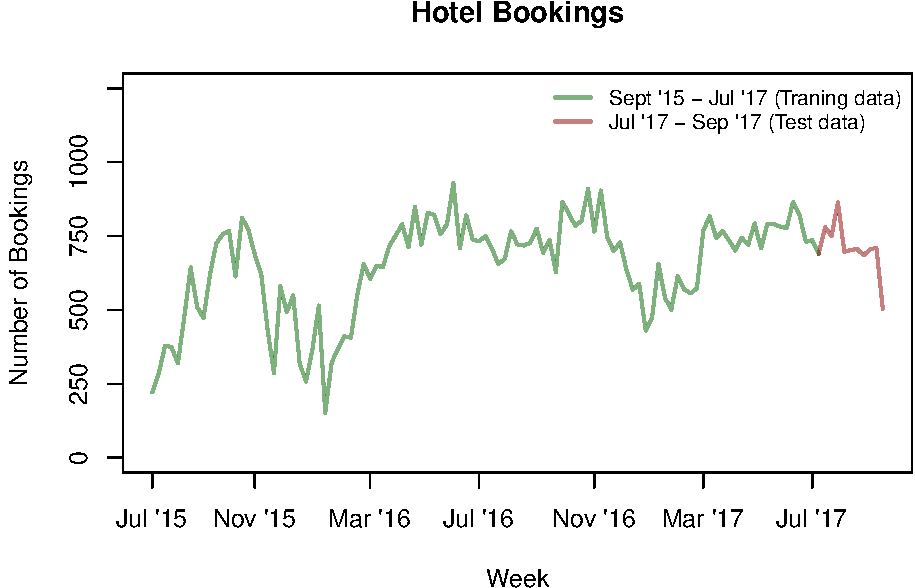
\includegraphics{bookings_forecast_files/figure-latex/unnamed-chunk-3-1} \end{center}

\(\;\)

The framework to predict the hotel demand for the remainder of 2017 is
as follows:

\begin{itemize}
\tightlist
\item
  transform non-stationary data to stationary data
\item
  fit a stationary model
\item
  forecast
\item
  add non-stationarity back
\end{itemize}

Data with a trend, change points, heteroscedasticity, or seasonality
indicate non-stationarity. To better identify non-stationary components,
let's decompose the data into its components.

\begin{Shaded}
\begin{Highlighting}[]
\NormalTok{bookings.training <-}\StringTok{ }\KeywordTok{head}\NormalTok{(bookings, }\DecValTok{104}\NormalTok{)}
\NormalTok{bookings.ts <-}\StringTok{ }\KeywordTok{ts}\NormalTok{(bookings.training, }\DataTypeTok{frequency=}\DecValTok{52}\NormalTok{) }\CommentTok{# frequency is 52 since we have weekly data}
\NormalTok{bookings.decomposed =}\StringTok{ }\KeywordTok{decompose}\NormalTok{(bookings.ts, }\DataTypeTok{type =} \StringTok{"additive"}\NormalTok{)}
\KeywordTok{plot}\NormalTok{(bookings.decomposed)}
\end{Highlighting}
\end{Shaded}

\begin{center}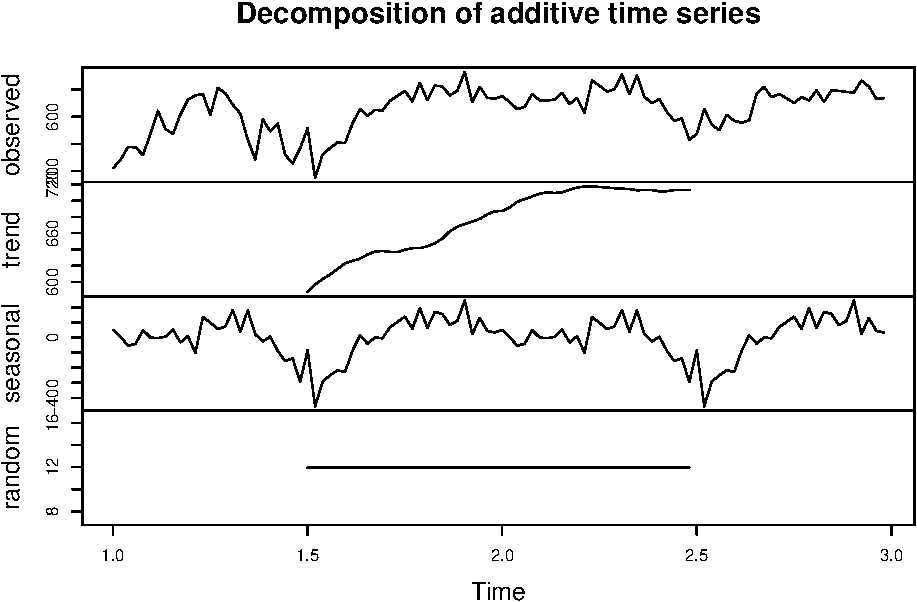
\includegraphics{bookings_forecast_files/figure-latex/unnamed-chunk-4-1} \end{center}

\begin{Shaded}
\begin{Highlighting}[]
\KeywordTok{acf}\NormalTok{(bookings.training, }\DataTypeTok{lag.max=}\DecValTok{104}\NormalTok{)}
\end{Highlighting}
\end{Shaded}

\begin{center}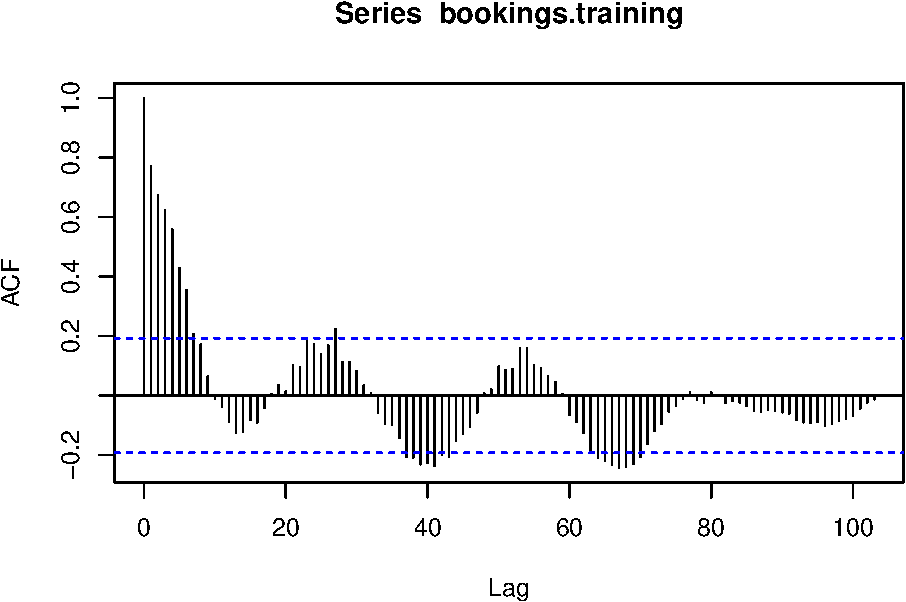
\includegraphics{bookings_forecast_files/figure-latex/unnamed-chunk-4-2} \end{center}

\(\;\)

From the plot, there is a clear trend and seasonlity.

There are a few options to remove the non-contant mean including
smoothing and differencing. First, we will consider an additive
Holt-Winters model.

\begin{Shaded}
\begin{Highlighting}[]
\NormalTok{hw.additive <-}\StringTok{ }\KeywordTok{HoltWinters}\NormalTok{(bookings.ts, }\DataTypeTok{seasonal=}\StringTok{"additive"}\NormalTok{)}
\NormalTok{randomcomponent =}\StringTok{ }\NormalTok{bookings.ts }\OperatorTok{-}\StringTok{ }\NormalTok{hw.additive}\OperatorTok{$}\NormalTok{fitted[,}\DecValTok{1}\NormalTok{]}
\KeywordTok{plot}\NormalTok{(randomcomponent)}
\end{Highlighting}
\end{Shaded}

\begin{center}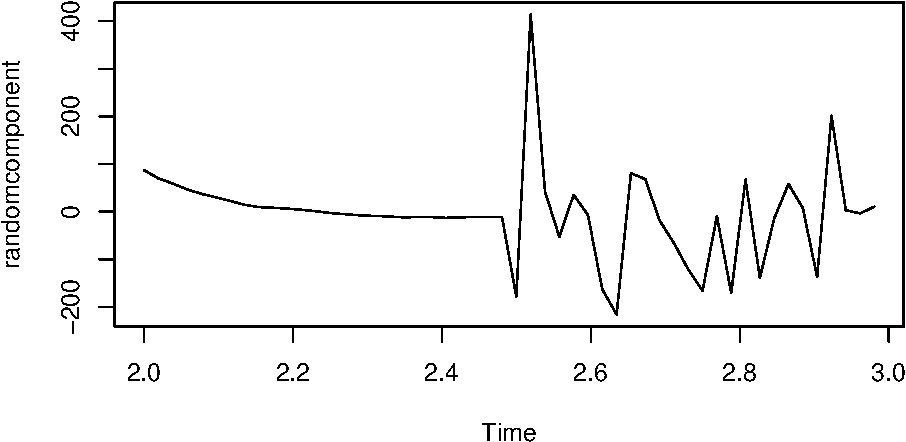
\includegraphics{bookings_forecast_files/figure-latex/unnamed-chunk-5-1} \end{center}

\begin{Shaded}
\begin{Highlighting}[]
\KeywordTok{acf}\NormalTok{(randomcomponent)}
\end{Highlighting}
\end{Shaded}

\begin{center}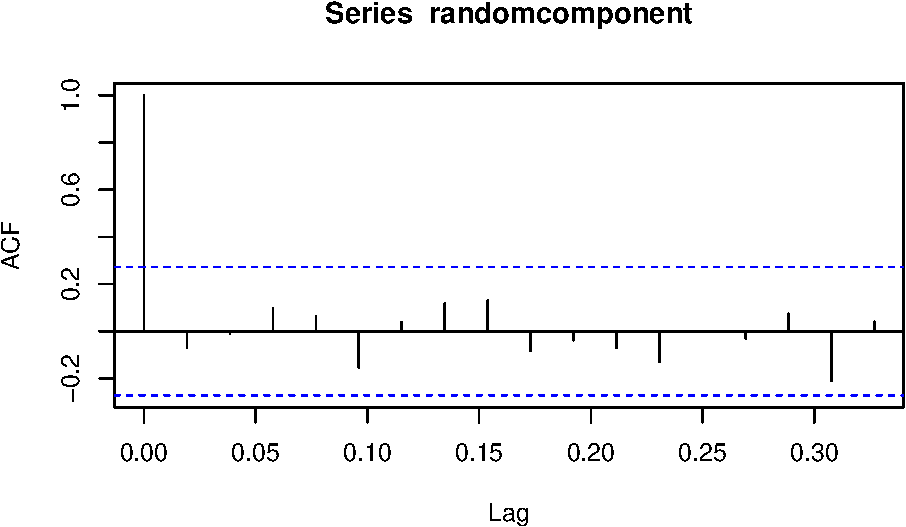
\includegraphics{bookings_forecast_files/figure-latex/unnamed-chunk-5-2} \end{center}

\(\;\)

There is no clear trend and/or seasonality in the random component,
hence we conclude that the series is stationary.

\newpage

\begin{Shaded}
\begin{Highlighting}[]
\NormalTok{hw.additive <-}\StringTok{ }\KeywordTok{HoltWinters}\NormalTok{(bookings.ts, }\DataTypeTok{seasonal=}\StringTok{"additive"}\NormalTok{)}
\NormalTok{pred.additive <-}\StringTok{ }\KeywordTok{predict}\NormalTok{(hw.additive, }\DataTypeTok{n.ahead=}\DecValTok{11}\NormalTok{)}

\NormalTok{bookings.training <-}\StringTok{ }\KeywordTok{head}\NormalTok{(bookings, }\DecValTok{105}\NormalTok{)}
\KeywordTok{plot}\NormalTok{(bookings.training,}
     \DataTypeTok{main =} \StringTok{"Hotel Bookings"}\NormalTok{,}
     \DataTypeTok{xlab =} \StringTok{"Week"}\NormalTok{,}
     \DataTypeTok{ylab =} \StringTok{"Number of Bookings"}\NormalTok{,}
     \DataTypeTok{xlim =} \KeywordTok{c}\NormalTok{(}\DecValTok{1}\NormalTok{, }\DecValTok{115}\NormalTok{),}
     \DataTypeTok{ylim =} \KeywordTok{c}\NormalTok{(}\DecValTok{0}\NormalTok{, }\DecValTok{1250}\NormalTok{),}
     \DataTypeTok{type =} \StringTok{"l"}\NormalTok{,}
     \DataTypeTok{lwd =} \DecValTok{2}\NormalTok{,}
     \DataTypeTok{col =} \KeywordTok{adjustcolor}\NormalTok{(}\StringTok{"darkgreen"}\NormalTok{, }\FloatTok{0.5}\NormalTok{),}
     \DataTypeTok{xaxt =} \StringTok{"n"}\NormalTok{,}
     \DataTypeTok{yaxt =} \StringTok{"n"}\NormalTok{)}

\KeywordTok{lines}\NormalTok{(}\DataTypeTok{y =}\NormalTok{ bookings.test,}
      \DataTypeTok{x =} \DecValTok{105}\OperatorTok{:}\DecValTok{115}\NormalTok{,}
      \DataTypeTok{lwd =} \DecValTok{2}\NormalTok{,}
      \DataTypeTok{col =} \KeywordTok{adjustcolor}\NormalTok{(}\StringTok{"darkred"}\NormalTok{, }\FloatTok{0.5}\NormalTok{))}

\KeywordTok{lines}\NormalTok{(}\DataTypeTok{y =}\NormalTok{ pred.additive,}
      \DataTypeTok{x =} \DecValTok{105}\OperatorTok{:}\DecValTok{115}\NormalTok{,}
      \DataTypeTok{lwd =} \DecValTok{2}\NormalTok{,}
      \DataTypeTok{col =} \KeywordTok{adjustcolor}\NormalTok{(}\StringTok{"darkblue"}\NormalTok{, }\FloatTok{0.5}\NormalTok{))}

\KeywordTok{axis}\NormalTok{(}\DataTypeTok{side =} \DecValTok{1}\NormalTok{, }\DataTypeTok{at =} \KeywordTok{c}\NormalTok{(}\DecValTok{1}\NormalTok{,}\DecValTok{17}\NormalTok{,}\DecValTok{35}\NormalTok{,}\DecValTok{52}\NormalTok{,}\DecValTok{70}\NormalTok{,}\DecValTok{87}\NormalTok{,}\DecValTok{104}\NormalTok{,}\DecValTok{122}\NormalTok{),}
     \DataTypeTok{labels =} \KeywordTok{c}\NormalTok{(}\StringTok{"Jul '15"}\NormalTok{,}\StringTok{"Nov '15"}\NormalTok{,}\StringTok{"Mar '16"}\NormalTok{,}\StringTok{"Jul '16"}\NormalTok{,}\StringTok{"Nov '16"}\NormalTok{,}\StringTok{"Mar '17"}\NormalTok{,}\StringTok{"Jul '17"}\NormalTok{,}\StringTok{"Nov '17"}\NormalTok{))}

\KeywordTok{axis}\NormalTok{(}\DataTypeTok{side =} \DecValTok{2}\NormalTok{, }\DataTypeTok{at =}\NormalTok{ (}\DecValTok{250}\OperatorTok{*}\DecValTok{0}\OperatorTok{:}\DecValTok{5}\NormalTok{), }\DataTypeTok{labels =} \KeywordTok{c}\NormalTok{(}\StringTok{"0"}\NormalTok{,}\StringTok{"250"}\NormalTok{,}\StringTok{"500"}\NormalTok{,}\StringTok{"750"}\NormalTok{,}\StringTok{"1000"}\NormalTok{, }\StringTok{"1250"}\NormalTok{))}

\KeywordTok{legend}\NormalTok{(}\StringTok{"topright"}\NormalTok{,}
       \DataTypeTok{lwd =} \DecValTok{2}\NormalTok{,}
       \DataTypeTok{bty =} \StringTok{"n"}\NormalTok{,}
       \DataTypeTok{cex =} \FloatTok{0.8}\NormalTok{,}
       \DataTypeTok{col =} \KeywordTok{c}\NormalTok{(}\KeywordTok{adjustcolor}\NormalTok{(}\StringTok{"darkgreen"}\NormalTok{, }\FloatTok{0.5}\NormalTok{), }\KeywordTok{adjustcolor}\NormalTok{(}\StringTok{"darkred"}\NormalTok{, }\FloatTok{0.5}\NormalTok{), }\KeywordTok{adjustcolor}\NormalTok{(}\StringTok{"darkblue"}\NormalTok{, }\FloatTok{0.5}\NormalTok{)),}
       \DataTypeTok{legend =} \KeywordTok{c}\NormalTok{(}\StringTok{"Sept '15 - Jul '17 (Training data)"}\NormalTok{, }\StringTok{"Jul '17 - Sep '17 (Training data)"}\NormalTok{, }\StringTok{"Jul '17 - Sep '17 (HW Smoothing)"}\NormalTok{),)}
\end{Highlighting}
\end{Shaded}

\begin{center}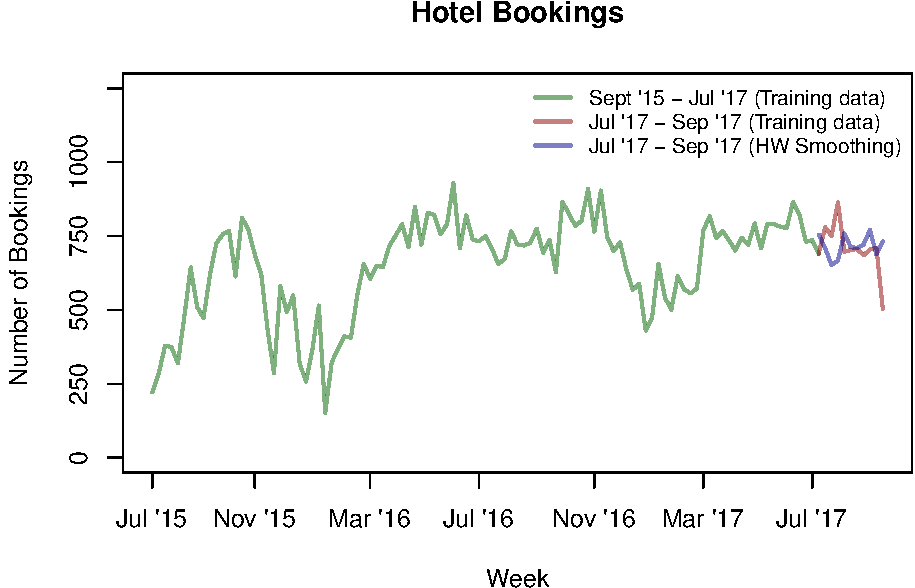
\includegraphics{bookings_forecast_files/figure-latex/unnamed-chunk-6-1} \end{center}

\(\;\)

And the \(SSE_{train}\) is 119812.8.

\begin{Shaded}
\begin{Highlighting}[]
\KeywordTok{sum}\NormalTok{((bookings.test}\OperatorTok{-}\NormalTok{pred.additive)}\OperatorTok{^}\DecValTok{2}\NormalTok{)}
\end{Highlighting}
\end{Shaded}

\begin{verbatim}
## [1] 119812.8
\end{verbatim}

\(\;\)

For differencing, we'll propose SARIMA models. Given the acf shows
periodicity, we first perform a one time regular differencing and, if
necessary, one time seasonal differencing.

\begin{Shaded}
\begin{Highlighting}[]
\KeywordTok{par}\NormalTok{(}\DataTypeTok{mfrow=}\KeywordTok{c}\NormalTok{(}\DecValTok{1}\NormalTok{,}\DecValTok{3}\NormalTok{))}

\NormalTok{bookings.training <-}\StringTok{ }\KeywordTok{head}\NormalTok{(bookings, }\DecValTok{104}\NormalTok{)}
\NormalTok{regdiff.bookings <-}\StringTok{ }\KeywordTok{diff}\NormalTok{(bookings.training, }\DataTypeTok{differences=}\DecValTok{1}\NormalTok{)}
\KeywordTok{plot}\NormalTok{(regdiff.bookings, }\DataTypeTok{type=}\StringTok{"l"}\NormalTok{)}
\KeywordTok{acf}\NormalTok{(regdiff.bookings, }\DataTypeTok{lag.max=}\DecValTok{52}\NormalTok{, }\DataTypeTok{main=}\StringTok{"Regular Differencing Once"}\NormalTok{)}
\KeywordTok{pacf}\NormalTok{(regdiff.bookings, }\DataTypeTok{lag.max=}\DecValTok{52}\NormalTok{)}
\end{Highlighting}
\end{Shaded}

\begin{center}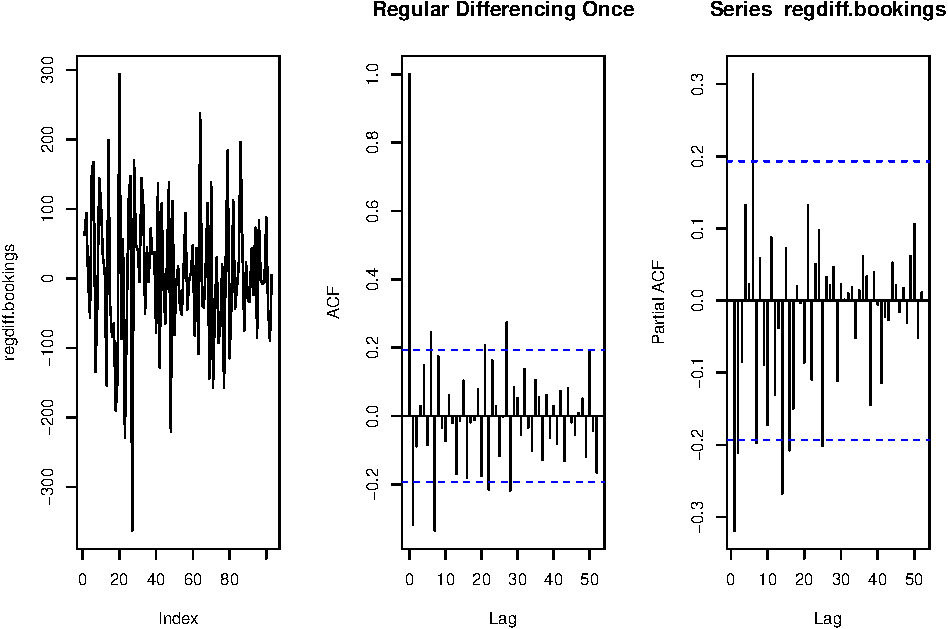
\includegraphics{bookings_forecast_files/figure-latex/unnamed-chunk-8-1} \end{center}

There is no linear decay and/or periodicity left, so we stop here. The
times series plot of the differenced series above shows no sign of trend
and/or seasonality either.

Next, we propose models for the stationary data and perform full
residuals diagnostics for the proposed ARIMA models.

\begin{itemize}
\tightlist
\item
  Model 1: the ACF has an exponential decay and the PACF cuts off after
  lag 6, so we consider ARIMA(6,1,0).
\item
  Model 2: the PACF has an exponential decay and the ACF cuts off after
  lag 7, so we consider ARIMA(0,1,7).
\item
  Model 3: since in models 1 and 2 we justified exponential decay on the
  ACF and PACF, it could be exponential decay on both, so we consider
  ARIMA(1,1,1).
\end{itemize}

\newpage

\hypertarget{model-1-arima6-1-0}{%
\subsection{Model 1: ARIMA(6, 1, 0)}\label{model-1-arima6-1-0}}

\begin{Shaded}
\begin{Highlighting}[]
\KeywordTok{library}\NormalTok{(astsa)}

\NormalTok{model1 <-}\StringTok{ }\KeywordTok{sarima}\NormalTok{(bookings.training, }\DataTypeTok{p=}\DecValTok{6}\NormalTok{, }\DataTypeTok{d=}\DecValTok{1}\NormalTok{, }\DataTypeTok{q=}\DecValTok{0}\NormalTok{, }\DataTypeTok{details =} \OtherTok{TRUE}\NormalTok{)}
\end{Highlighting}
\end{Shaded}

\begin{verbatim}
## initial  value 4.668937 
## iter   2 value 4.557498
## iter   3 value 4.516215
## iter   4 value 4.514142
## iter   5 value 4.513256
## iter   6 value 4.513223
## iter   7 value 4.513217
## iter   8 value 4.513216
## iter   9 value 4.513216
## iter   9 value 4.513216
## iter   9 value 4.513216
## final  value 4.513216 
## converged
## initial  value 4.531137 
## iter   2 value 4.528791
## iter   3 value 4.527646
## iter   4 value 4.527613
## iter   5 value 4.527545
## iter   6 value 4.527543
## iter   7 value 4.527542
## iter   7 value 4.527542
## iter   7 value 4.527542
## final  value 4.527542 
## converged
\end{verbatim}

\begin{center}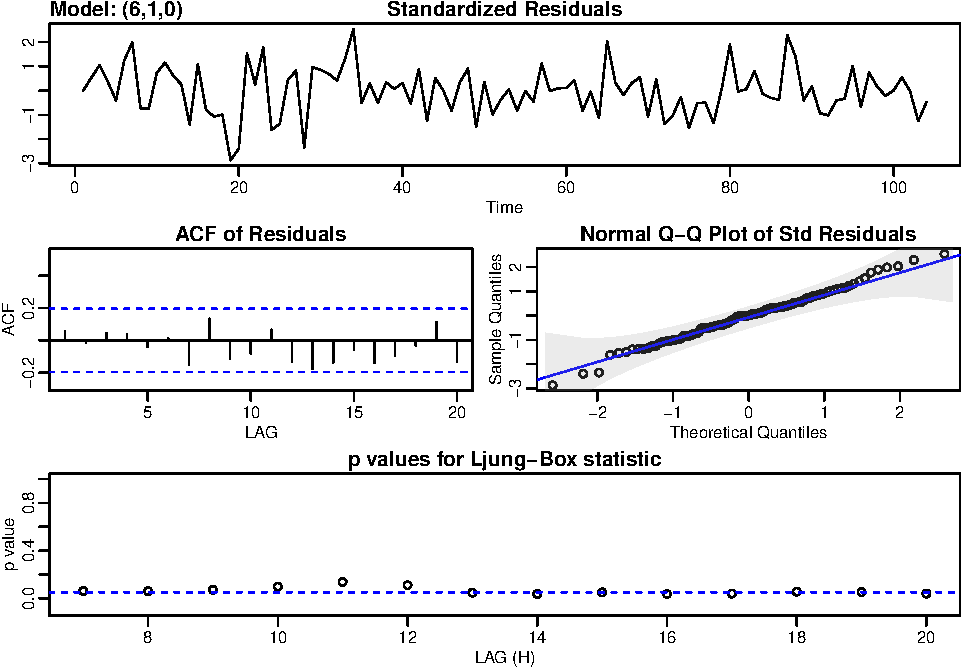
\includegraphics{bookings_forecast_files/figure-latex/unnamed-chunk-9-1} \end{center}

\begin{Shaded}
\begin{Highlighting}[]
\NormalTok{seg <-}\StringTok{ }\KeywordTok{c}\NormalTok{(}\KeywordTok{rep}\NormalTok{(}\DecValTok{1}\OperatorTok{:}\DecValTok{6}\NormalTok{, }\DataTypeTok{each=}\DecValTok{16}\NormalTok{), }\KeywordTok{rep}\NormalTok{(}\DecValTok{7}\NormalTok{,}\DecValTok{8}\NormalTok{))}
\KeywordTok{fligner.test}\NormalTok{(model1}\OperatorTok{$}\NormalTok{fit}\OperatorTok{$}\NormalTok{residuals, seg)}
\end{Highlighting}
\end{Shaded}

\begin{verbatim}
## 
##  Fligner-Killeen test of homogeneity of variances
## 
## data:  model1$fit$residuals and seg
## Fligner-Killeen:med chi-squared = 12.193, df = 6, p-value =
## 0.05779
\end{verbatim}

\begin{Shaded}
\begin{Highlighting}[]
\KeywordTok{shapiro.test}\NormalTok{(model1}\OperatorTok{$}\NormalTok{fit}\OperatorTok{$}\NormalTok{residuals)}
\end{Highlighting}
\end{Shaded}

\begin{verbatim}
## 
##  Shapiro-Wilk normality test
## 
## data:  model1$fit$residuals
## W = 0.99287, p-value = 0.8653
\end{verbatim}

\(\;\)

\begin{itemize}
\tightlist
\item
  ARIMA(6, 1, 0)

  \begin{itemize}
  \tightlist
  \item
    Homoscedasticity: the time series of the residuals appears to have
    no trend and the p-value of Fligner's test (0.05779) confirms the
    validity of homoscedasticity.
  \item
    Normality: a few points in the QQplot slightly deviate from the
    straight line resulting in the p-value of Shapiro-Wilk's test
    (0.8653). The normality assumption is valid.
  \item
    White Noise: a few p-values of Ljung-Box statistic are below the
    threshold which raises concerns about the independence of the
    residuals.
  \end{itemize}
\end{itemize}

\newpage

\hypertarget{model-2-arima0-1-7}{%
\subsection{Model 2: ARIMA(0, 1, 7)}\label{model-2-arima0-1-7}}

\(\;\)

\begin{Shaded}
\begin{Highlighting}[]
\KeywordTok{library}\NormalTok{(astsa)}

\NormalTok{model2 <-}\StringTok{ }\KeywordTok{sarima}\NormalTok{(bookings.training, }\DataTypeTok{p=}\DecValTok{0}\NormalTok{, }\DataTypeTok{d=}\DecValTok{2}\NormalTok{, }\DataTypeTok{q=}\DecValTok{1}\NormalTok{, }\DataTypeTok{details =} \OtherTok{TRUE}\NormalTok{)}
\end{Highlighting}
\end{Shaded}

\begin{verbatim}
## initial  value 5.156737 
## iter   2 value 4.850525
## iter   3 value 4.804598
## iter   4 value 4.765159
## iter   5 value 4.730889
## iter   6 value 4.721112
## iter   7 value 4.703716
## iter   8 value 4.702832
## iter   9 value 4.702815
## iter  10 value 4.702814
## iter  10 value 4.702814
## final  value 4.702814 
## converged
## initial  value 4.703056 
## iter   2 value 4.697225
## iter   3 value 4.695194
## iter   4 value 4.695076
## iter   5 value 4.695073
## iter   6 value 4.695072
## iter   6 value 4.695072
## iter   6 value 4.695072
## final  value 4.695072 
## converged
\end{verbatim}

\begin{center}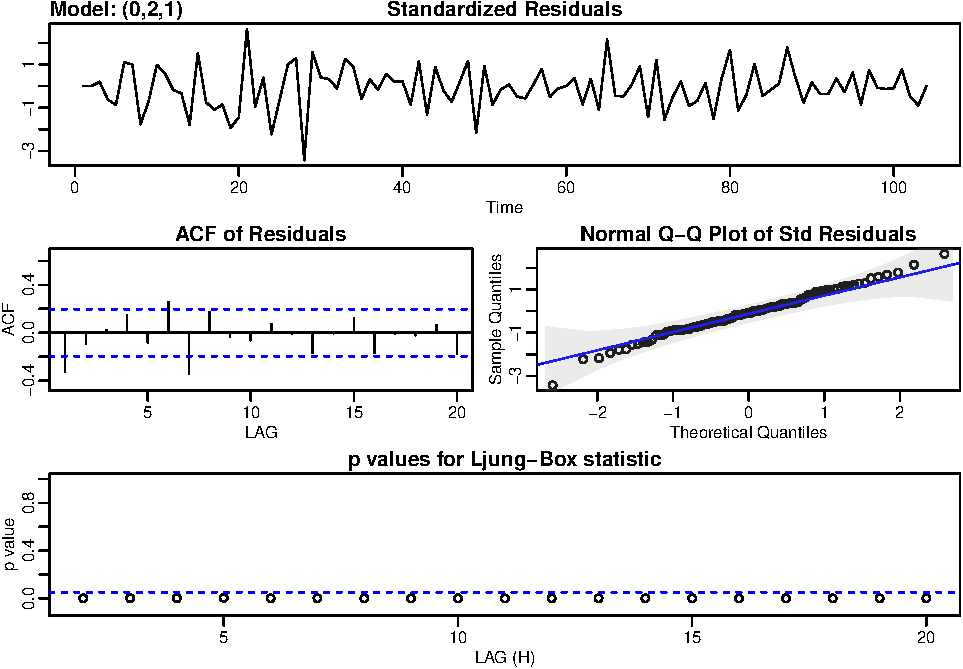
\includegraphics{bookings_forecast_files/figure-latex/unnamed-chunk-10-1} \end{center}

\begin{Shaded}
\begin{Highlighting}[]
\NormalTok{seg <-}\StringTok{ }\KeywordTok{c}\NormalTok{(}\KeywordTok{rep}\NormalTok{(}\DecValTok{1}\OperatorTok{:}\DecValTok{6}\NormalTok{, }\DataTypeTok{each=}\DecValTok{16}\NormalTok{), }\KeywordTok{rep}\NormalTok{(}\DecValTok{7}\NormalTok{,}\DecValTok{8}\NormalTok{))}
\KeywordTok{fligner.test}\NormalTok{(model2}\OperatorTok{$}\NormalTok{fit}\OperatorTok{$}\NormalTok{residuals, seg)}
\end{Highlighting}
\end{Shaded}

\begin{verbatim}
## 
##  Fligner-Killeen test of homogeneity of variances
## 
## data:  model2$fit$residuals and seg
## Fligner-Killeen:med chi-squared = 15.533, df = 6, p-value =
## 0.01649
\end{verbatim}

\begin{Shaded}
\begin{Highlighting}[]
\KeywordTok{shapiro.test}\NormalTok{(model2}\OperatorTok{$}\NormalTok{fit}\OperatorTok{$}\NormalTok{residuals)}
\end{Highlighting}
\end{Shaded}

\begin{verbatim}
## 
##  Shapiro-Wilk normality test
## 
## data:  model2$fit$residuals
## W = 0.99094, p-value = 0.7161
\end{verbatim}

\(\;\)

\begin{itemize}
\tightlist
\item
  ARIMA(0, 1, 7)

  \begin{itemize}
  \tightlist
  \item
    Homoscedasticity: the time series of the residuals has no trend and
    the p-value of Fligner's test (0.01649) does not raise much concern.
  \item
    Normality: the points in the QQplot don't deviate from the straight
    line resulting in the large p-value of Shapiro-Wilk's test (0.7161).
    The normality assumption of the residuals is valid.
  \item
    White Noise: the p-values of the Ljung-Box statistic are below the
    threshold and there is concern in the ACF plot. We can safely
    conclude the residuals are not realizations of white noise.
  \end{itemize}
\end{itemize}

\(\;\)

\hypertarget{model-3-arima1-1-1}{%
\subsection{Model 3: ARIMA(1, 1, 1)}\label{model-3-arima1-1-1}}

\(\;\)

\begin{Shaded}
\begin{Highlighting}[]
\KeywordTok{library}\NormalTok{(astsa)}

\NormalTok{model3 <-}\StringTok{ }\KeywordTok{sarima}\NormalTok{(bookings.training, }\DataTypeTok{p=}\DecValTok{1}\NormalTok{, }\DataTypeTok{d=}\DecValTok{2}\NormalTok{, }\DataTypeTok{q=}\DecValTok{1}\NormalTok{, }\DataTypeTok{details =} \OtherTok{TRUE}\NormalTok{)}
\end{Highlighting}
\end{Shaded}

\begin{verbatim}
## initial  value 5.161506 
## iter   2 value 4.774085
## iter   3 value 4.742362
## iter   4 value 4.723250
## iter   5 value 4.711304
## iter   6 value 4.701406
## iter   7 value 4.685902
## iter   8 value 4.676268
## iter   9 value 4.673973
## iter  10 value 4.673110
## iter  11 value 4.672555
## iter  12 value 4.672493
## iter  13 value 4.672490
## iter  13 value 4.672490
## iter  13 value 4.672490
## final  value 4.672490 
## converged
## initial  value 4.662495 
## iter   2 value 4.651553
## iter   3 value 4.644807
## iter   4 value 4.644586
## iter   5 value 4.644505
## iter   6 value 4.644497
## iter   7 value 4.644496
## iter   8 value 4.644495
## iter   9 value 4.644494
## iter   9 value 4.644494
## iter   9 value 4.644494
## final  value 4.644494 
## converged
\end{verbatim}

\begin{center}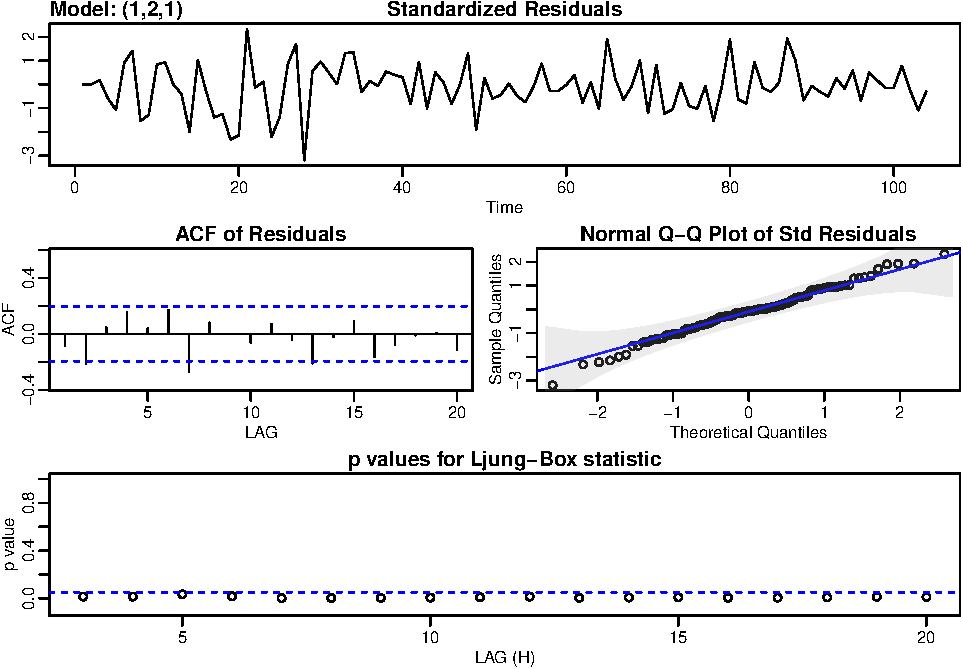
\includegraphics{bookings_forecast_files/figure-latex/unnamed-chunk-11-1} \end{center}

\begin{Shaded}
\begin{Highlighting}[]
\NormalTok{seg <-}\StringTok{ }\KeywordTok{c}\NormalTok{(}\KeywordTok{rep}\NormalTok{(}\DecValTok{1}\OperatorTok{:}\DecValTok{6}\NormalTok{, }\DataTypeTok{each=}\DecValTok{16}\NormalTok{), }\KeywordTok{rep}\NormalTok{(}\DecValTok{7}\NormalTok{,}\DecValTok{8}\NormalTok{))}
\KeywordTok{fligner.test}\NormalTok{(model3}\OperatorTok{$}\NormalTok{fit}\OperatorTok{$}\NormalTok{residuals, seg)}
\end{Highlighting}
\end{Shaded}

\begin{verbatim}
## 
##  Fligner-Killeen test of homogeneity of variances
## 
## data:  model3$fit$residuals and seg
## Fligner-Killeen:med chi-squared = 19.871, df = 6, p-value =
## 0.00292
\end{verbatim}

\begin{Shaded}
\begin{Highlighting}[]
\KeywordTok{shapiro.test}\NormalTok{(model3}\OperatorTok{$}\NormalTok{fit}\OperatorTok{$}\NormalTok{residuals)}
\end{Highlighting}
\end{Shaded}

\begin{verbatim}
## 
##  Shapiro-Wilk normality test
## 
## data:  model3$fit$residuals
## W = 0.98941, p-value = 0.5889
\end{verbatim}

\(\;\)

\begin{itemize}
\tightlist
\item
  ARIMA(1, 1, 1)

  \begin{itemize}
  \tightlist
  \item
    Homoscedasticity: the time series of the residuals has no trend but
    the p-value of Fligner's test (0.00292) raises concern. The constant
    variance assumption is not valid.
  \item
    Normality: the points in the QQplot don't deviate from the straight
    line resulting in the large p-value of Shapiro-Wilk's test (0.5889).
    The normality assumption of the residuals is valid.
  \item
    White Noise: the p-values of the Ljung-Box statistic are below the
    threshold and there is concern in the ACF plot. We can safely
    conclude the residuals are not realizations of white noise.
  \end{itemize}
\end{itemize}

\newpage

Let's compare the three proposed ARIMA models in terms of their
prediction power using PRESS and MSE.

\begin{Shaded}
\begin{Highlighting}[]
\KeywordTok{par}\NormalTok{(}\DataTypeTok{mfrow=}\KeywordTok{c}\NormalTok{(}\DecValTok{3}\NormalTok{,}\DecValTok{1}\NormalTok{))}
\NormalTok{pred.model1 <-}\StringTok{ }\KeywordTok{sarima.for}\NormalTok{(bookings.training, }\DataTypeTok{n.ahead=}\DecValTok{11}\NormalTok{, }\DataTypeTok{p=}\DecValTok{6}\NormalTok{, }\DataTypeTok{d=}\DecValTok{1}\NormalTok{, }\DataTypeTok{q=}\DecValTok{0}\NormalTok{)}
\NormalTok{pred.model2 <-}\StringTok{ }\KeywordTok{sarima.for}\NormalTok{(bookings.training, }\DataTypeTok{n.ahead=}\DecValTok{11}\NormalTok{, }\DataTypeTok{p=}\DecValTok{0}\NormalTok{, }\DataTypeTok{d=}\DecValTok{1}\NormalTok{, }\DataTypeTok{q=}\DecValTok{7}\NormalTok{)}
\NormalTok{pred.model3 <-}\StringTok{ }\KeywordTok{sarima.for}\NormalTok{(bookings.training, }\DataTypeTok{n.ahead=}\DecValTok{11}\NormalTok{, }\DataTypeTok{p=}\DecValTok{1}\NormalTok{, }\DataTypeTok{d=}\DecValTok{1}\NormalTok{, }\DataTypeTok{q=}\DecValTok{1}\NormalTok{)}
\end{Highlighting}
\end{Shaded}

\begin{Shaded}
\begin{Highlighting}[]
\NormalTok{PRESS}\FloatTok{.1}\NormalTok{ <-}\StringTok{ }\KeywordTok{sum}\NormalTok{((pred.model1}\OperatorTok{$}\NormalTok{pred}\OperatorTok{-}\NormalTok{bookings.test)}\OperatorTok{^}\DecValTok{2}\NormalTok{)}
\NormalTok{PRESS}\FloatTok{.2}\NormalTok{ <-}\StringTok{ }\KeywordTok{sum}\NormalTok{((pred.model2}\OperatorTok{$}\NormalTok{pred}\OperatorTok{-}\NormalTok{bookings.test)}\OperatorTok{^}\DecValTok{2}\NormalTok{)}
\NormalTok{PRESS}\FloatTok{.3}\NormalTok{ <-}\StringTok{ }\KeywordTok{sum}\NormalTok{((pred.model3}\OperatorTok{$}\NormalTok{pred}\OperatorTok{-}\NormalTok{bookings.test)}\OperatorTok{^}\DecValTok{2}\NormalTok{)}

\NormalTok{tab =}\StringTok{ }\KeywordTok{rbind}\NormalTok{(}\DecValTok{1}\OperatorTok{:}\DecValTok{3}\NormalTok{, }\KeywordTok{c}\NormalTok{(PRESS}\FloatTok{.1}\NormalTok{, PRESS}\FloatTok{.2}\NormalTok{, PRESS}\FloatTok{.3}\NormalTok{))}
\KeywordTok{row.names}\NormalTok{(tab) =}\StringTok{ }\KeywordTok{c}\NormalTok{(}\StringTok{"ARIMA Model"}\NormalTok{, }\StringTok{"PRESS"}\NormalTok{)}
\KeywordTok{dimnames}\NormalTok{(tab)[[}\DecValTok{2}\NormalTok{]] =}\StringTok{ }\KeywordTok{rep}\NormalTok{(}\StringTok{""}\NormalTok{, }\DecValTok{3}\NormalTok{)}
\NormalTok{tab}
\end{Highlighting}
\end{Shaded}

\begin{verbatim}
##                                     
## ARIMA Model      1.0      2      3.0
## PRESS       123439.6 203711 150550.7
\end{verbatim}

\(\;\)

Based on the PRESS statistic, ARIMA(6, 1, 0) predicts the best.

\(\;\)

\begin{Shaded}
\begin{Highlighting}[]
\NormalTok{MSE}\FloatTok{.1}\NormalTok{ <-}\StringTok{ }\KeywordTok{sum}\NormalTok{((pred.model1}\OperatorTok{$}\NormalTok{pred}\OperatorTok{-}\NormalTok{bookings.test)}\OperatorTok{^}\DecValTok{2}\NormalTok{)}\OperatorTok{/}\DecValTok{3}
\NormalTok{MSE}\FloatTok{.2}\NormalTok{ <-}\StringTok{ }\KeywordTok{sum}\NormalTok{((pred.model1}\OperatorTok{$}\NormalTok{pred}\OperatorTok{-}\NormalTok{bookings.test)}\OperatorTok{^}\DecValTok{2}\NormalTok{)}\OperatorTok{/}\DecValTok{1}
\NormalTok{MSE}\FloatTok{.3}\NormalTok{ <-}\StringTok{ }\KeywordTok{sum}\NormalTok{((pred.model1}\OperatorTok{$}\NormalTok{pred}\OperatorTok{-}\NormalTok{bookings.test)}\OperatorTok{^}\DecValTok{2}\NormalTok{)}\OperatorTok{/}\DecValTok{2}

\NormalTok{tab =}\StringTok{ }\KeywordTok{rbind}\NormalTok{(}\DecValTok{1}\OperatorTok{:}\DecValTok{3}\NormalTok{, }\KeywordTok{c}\NormalTok{(MSE}\FloatTok{.1}\NormalTok{, MSE}\FloatTok{.2}\NormalTok{, MSE}\FloatTok{.3}\NormalTok{))}
\KeywordTok{row.names}\NormalTok{(tab) =}\StringTok{ }\KeywordTok{c}\NormalTok{(}\StringTok{"ARIMA Model"}\NormalTok{, }\StringTok{"MSE"}\NormalTok{)}
\KeywordTok{dimnames}\NormalTok{(tab)[[}\DecValTok{2}\NormalTok{]] =}\StringTok{ }\KeywordTok{rep}\NormalTok{(}\StringTok{""}\NormalTok{, }\DecValTok{3}\NormalTok{)}
\NormalTok{tab}
\end{Highlighting}
\end{Shaded}

\begin{verbatim}
##                                       
## ARIMA Model     1.00      2.0     3.00
## MSE         41146.53 123439.6 61719.79
\end{verbatim}

\(\;\)

Based on the MSE statistic which accounts for the number of parameters,
ARIMA(6, 1, 0) predicts the best.

We choose the superior model to be ARIMA(6, 1, 0).

Up until now, we have two models to predict (along with a 95\%
prediction interval) the hotel demand for the remainder of 2017.

\begin{itemize}
\tightlist
\item
  Holt-Winter Additive
\item
  ARIMA(6,1,0)
\end{itemize}

It appears that the Holt-Winters Additive model is superior in term of
SSE, so that is the model we will choose. Note, we could spend more time
finding a better SARIMA model for the time series.

\begin{Shaded}
\begin{Highlighting}[]
\NormalTok{bookings.ts <-}\StringTok{ }\KeywordTok{ts}\NormalTok{(bookings, }\DataTypeTok{frequency=}\DecValTok{52}\NormalTok{)}
\NormalTok{final.model <-}\StringTok{ }\KeywordTok{HoltWinters}\NormalTok{(bookings.ts, }\DataTypeTok{seasonal=}\StringTok{"additive"}\NormalTok{)}
\NormalTok{pred.additive <-}\StringTok{ }\KeywordTok{predict}\NormalTok{(final.model, }\DataTypeTok{n.ahead=}\DecValTok{17}\NormalTok{, }\DataTypeTok{prediction.interval =} \OtherTok{TRUE}\NormalTok{)}
\NormalTok{fit <-}\StringTok{ }\NormalTok{pred.additive[,}\DecValTok{1}\NormalTok{]}
\NormalTok{lwr <-}\StringTok{ }\NormalTok{pred.additive[,}\DecValTok{2}\NormalTok{]}
\NormalTok{upr <-}\StringTok{ }\NormalTok{pred.additive[,}\DecValTok{3}\NormalTok{]}
\end{Highlighting}
\end{Shaded}

\begin{Shaded}
\begin{Highlighting}[]
\KeywordTok{plot}\NormalTok{(bookings,}
     \DataTypeTok{main =} \StringTok{"Hotel Bookings"}\NormalTok{,}
     \DataTypeTok{xlab =} \StringTok{"Week"}\NormalTok{,}
     \DataTypeTok{ylab =} \StringTok{"Total Bookings"}\NormalTok{,}
     \DataTypeTok{xlim =} \KeywordTok{c}\NormalTok{(}\DecValTok{1}\NormalTok{, }\DecValTok{132}\NormalTok{),}
     \DataTypeTok{ylim =} \KeywordTok{c}\NormalTok{(}\DecValTok{0}\NormalTok{, }\DecValTok{1250}\NormalTok{),}
     \DataTypeTok{type =} \StringTok{"l"}\NormalTok{,}
     \DataTypeTok{col =} \KeywordTok{adjustcolor}\NormalTok{(}\StringTok{"darkgreen"}\NormalTok{, }\FloatTok{0.5}\NormalTok{),}
     \DataTypeTok{xaxt =} \StringTok{"n"}\NormalTok{,}
     \DataTypeTok{yaxt =} \StringTok{"n"}\NormalTok{)}

\KeywordTok{lines}\NormalTok{(}\DataTypeTok{y =} \KeywordTok{c}\NormalTok{(}\KeywordTok{tail}\NormalTok{(bookings, }\DecValTok{1}\NormalTok{),fit),}
      \DataTypeTok{x =} \DecValTok{115}\OperatorTok{:}\DecValTok{132}\NormalTok{,}
      \DataTypeTok{type =}\StringTok{"l"}\NormalTok{,}
      \DataTypeTok{pch =} \DecValTok{19}\NormalTok{,}
      \DataTypeTok{col =} \KeywordTok{adjustcolor}\NormalTok{(}\StringTok{"red"}\NormalTok{, }\FloatTok{0.5}\NormalTok{))}

\KeywordTok{lines}\NormalTok{(}\DataTypeTok{y =}\NormalTok{ lwr,}
      \DataTypeTok{x =} \DecValTok{116}\OperatorTok{:}\DecValTok{132}\NormalTok{,}
      \DataTypeTok{type =}\StringTok{"l"}\NormalTok{,}
      \DataTypeTok{pch =} \DecValTok{19}\NormalTok{,}
      \DataTypeTok{col =} \KeywordTok{adjustcolor}\NormalTok{(}\StringTok{"grey"}\NormalTok{, }\FloatTok{0.5}\NormalTok{))}

\KeywordTok{lines}\NormalTok{(}\DataTypeTok{y =}\NormalTok{ upr,}
      \DataTypeTok{x =} \DecValTok{116}\OperatorTok{:}\DecValTok{132}\NormalTok{,}
      \DataTypeTok{type =}\StringTok{"l"}\NormalTok{,}
      \DataTypeTok{pch =} \DecValTok{19}\NormalTok{,}
      \DataTypeTok{col =} \KeywordTok{adjustcolor}\NormalTok{(}\StringTok{"grey"}\NormalTok{, }\FloatTok{0.5}\NormalTok{))}

\KeywordTok{polygon}\NormalTok{(}\KeywordTok{c}\NormalTok{(}\DecValTok{116}\OperatorTok{:}\DecValTok{132}\NormalTok{, }\KeywordTok{rev}\NormalTok{(}\DecValTok{116}\OperatorTok{:}\DecValTok{132}\NormalTok{)), }\KeywordTok{c}\NormalTok{(lwr, }\KeywordTok{rev}\NormalTok{(upr)), }\DataTypeTok{col =} \StringTok{"#69696930"}\NormalTok{, }\DataTypeTok{border =} \OtherTok{NA}\NormalTok{)}

\KeywordTok{axis}\NormalTok{(}\DataTypeTok{side =} \DecValTok{1}\NormalTok{, }\DataTypeTok{at =} \KeywordTok{c}\NormalTok{(}\DecValTok{1}\NormalTok{,}\DecValTok{17}\NormalTok{,}\DecValTok{35}\NormalTok{,}\DecValTok{52}\NormalTok{,}\DecValTok{70}\NormalTok{,}\DecValTok{87}\NormalTok{,}\DecValTok{104}\NormalTok{,}\DecValTok{122}\NormalTok{),}
     \DataTypeTok{labels =} \KeywordTok{c}\NormalTok{(}\StringTok{"Jul '15"}\NormalTok{,}\StringTok{"Nov '15"}\NormalTok{,}\StringTok{"Mar '16"}\NormalTok{,}\StringTok{"Jul '16"}\NormalTok{,}\StringTok{"Nov '16"}\NormalTok{,}\StringTok{"Mar '17"}\NormalTok{,}\StringTok{"Jul '17"}\NormalTok{,}\StringTok{"Nov '17"}\NormalTok{))}

\KeywordTok{axis}\NormalTok{(}\DataTypeTok{side =} \DecValTok{2}\NormalTok{, }\DataTypeTok{at =}\NormalTok{ (}\DecValTok{250}\OperatorTok{*}\DecValTok{0}\OperatorTok{:}\DecValTok{5}\NormalTok{), }\DataTypeTok{labels =} \KeywordTok{c}\NormalTok{(}\StringTok{"0"}\NormalTok{,}\StringTok{"250"}\NormalTok{,}\StringTok{"500"}\NormalTok{,}\StringTok{"750"}\NormalTok{,}\StringTok{"1000"}\NormalTok{, }\StringTok{"1250"}\NormalTok{))}

\KeywordTok{legend}\NormalTok{(}\StringTok{"topright"}\NormalTok{,}
       \DataTypeTok{lwd =} \DecValTok{2}\NormalTok{,}
       \DataTypeTok{bty =} \StringTok{"n"}\NormalTok{,}
       \DataTypeTok{cex =} \FloatTok{0.8}\NormalTok{,}
       \DataTypeTok{col =} \KeywordTok{c}\NormalTok{(}\KeywordTok{adjustcolor}\NormalTok{(}\StringTok{"darkgreen"}\NormalTok{, }\FloatTok{0.5}\NormalTok{), }\KeywordTok{adjustcolor}\NormalTok{(}\StringTok{"darkred"}\NormalTok{, }\FloatTok{0.5}\NormalTok{)),}
       \DataTypeTok{legend =} \KeywordTok{c}\NormalTok{(}\StringTok{"Sept '15 - Sept '17 (Bookings)"}\NormalTok{, }\StringTok{"Sept '17 - Dec '17 (Prediction)"}\NormalTok{),)}
\end{Highlighting}
\end{Shaded}

\begin{center}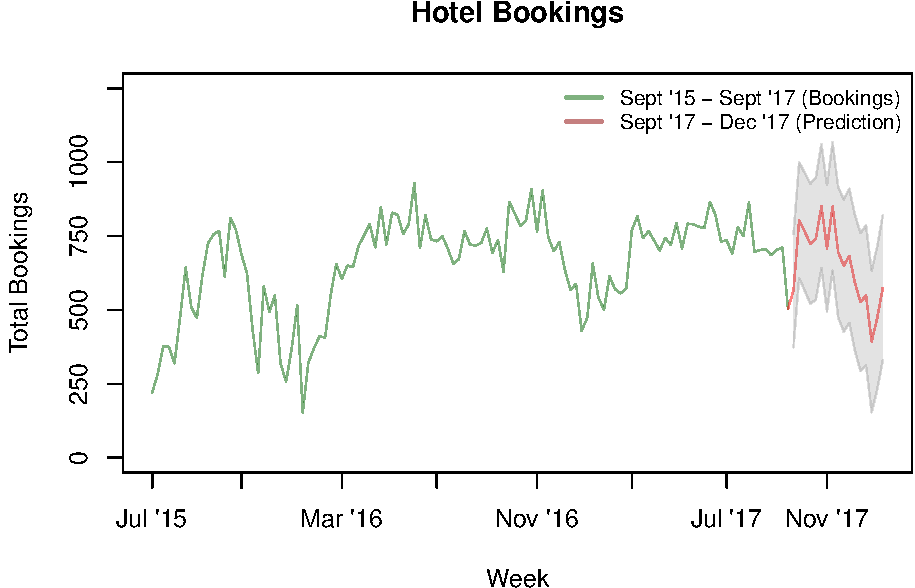
\includegraphics{bookings_forecast_files/figure-latex/unnamed-chunk-15-1} \end{center}

In the future, we could forecast by hotel vs.~resort. Furthermore,
instead of weekly forecast, we could forecast by day, month, or quarter
and for a specific region.


\end{document}
